%%%%%%%%%%%%%%%%%%%%%%%%%%%%%%%%%%%%%%%%%%%%%%%%%%%
%
%  Author: Jacob Vaughn
%  
%  Last Updated: 3/8/2024
%
%%%%%%%%%%%%%%%%%%%%%%%%%%%%%%%%%%%%%%%%%%%%%%%%%%%

%%%%%%%%%%%%%%%%%%%%%%%%%%%%%%%%%%%%%%%%%%%%%%%%%%%%%%%%%%%%%%%%%%%%%%
%%               EXPERIMENTAL APPROACH & OBJECTIVES
%%%%%%%%%%%%%%%%%%%%%%%%%%%%%%%%%%%%%%%%%%%%%%%%%%%%%%%%%%%%%%%%%%%%%

\chapter{EXPERIMENTAL APPROACH \& OBJECTIVES}

Following the completed installation and calibration discussed above, each of the three primary objectives will be accomplished or demonstrated sequentially. First, the improved experimental control and efficiency as a result of the above ACE2.0 design will be demonstrated by establishing and verifying the feedback-controlled active Mach variation and selection capability as well as the Reynolds number control scheme, if implemented. Second, the freestream flow produced by the calibrated nozzle will be characterized in terms of freestream flow uniformity and disturbance levels with uncertainty quantification and an exploration hysteresis. Third, the flow parameter control capabilities will be demonstrated in a proof of concept experiment of shock interactions during a Mach trajectory and any potential hysteresis exhibited. As a result of this work, the foundation will be set for future researchers to explore dynamic hypersonic aerodynamic in a more sophisticated and efficient manner with the control capabilities of ACE2.0.

\section{Improved Experimental Control and Efficiency} 

The overall objective here is to establish and substantiate the mechanisms of ACE2.0 that allow greater control of the tunnel input parameters for both more efficient and dynamic experiments. The primary design objective of ACE2.0 was to enable active Mach number control during a run, which alone provides many key experimental advantages. However, there is still much to be desired with the parameter control capabilities to achieve full aerodynamic similarity for any flight trajectory. Thus, more precise control methods for Mach number and Reynolds number will be explored through the following objectives.

\subsection{Feedback-Controlled Active Mach Number Variation and Selection}

As stated, the primary design objective of ACE2.0 was to enable active control of the Mach number, but this capability will be taken one step further to accurately maintain the desired Mach number once set. During a tunnel run, the Mach number may vary because both pressure and thermal loads can cause the throat height to vary. Current experience shows that the Mach number can vary by up to 5\%. The goal of this work is to implement active feedback control and reduce this error to less than 0.5\%.

The general approach for this feedback control is straightforward by designing a PID controller with an input of the measured Mach number and output of actuator position or velocity. The measured Mach number is calculated from the measured stagnation pressure and static pressure by solving the isentropic relation:
\begin{equation} 
    M = \sqrt{\frac{2}{\gamma - 1} \left[\left(\frac{P_0}{P}\right)^{\frac{\gamma - 1}{\gamma}} - 1\right]}
\end{equation}

\noindent The relationship between the throat height and the Mach number is given by:
\begin{equation}
    \frac{A^*}{A} = \frac{h^*}{h_{\mathrm{exit}}} = M \left[ \left( \frac{2}{\gamma+1}  \right) \left( 1 + \frac{\gamma-1}{2} M^2  \right) \right]^{-\frac{\gamma+1}{2(\gamma-1)} }
\end{equation}

\noindent This is then subtracted from the set throat height to get the error signal for the PID transfer function:
\begin{equation}
    E(s) = h_{\mathrm{set}} - H(s)
\end{equation}

There are many design options for PID controllers depending on the desired performance characteristics. The standard approach is simply a PI controller due to the derivative action amplifying measurement noise and potential causing instability \cite{fung}. However, the derivative effect of limiting overshoot and settling time is desirable, so it will not be neglected entirely. One final option is to add high frequency filtering into the derivative term to mitigate the effects of measurement noise. Each of these options will be explored, and the following equations show the transfer functions for PI, PID, and PID with high frequency noise filtering respectively:
\begin{subequations}
    \begin{align}
        G(s) = \frac{H(s)}{E(s)} &= K \left(1 + \frac{1}{T_i s}\right) \label{eq:M-PI}\\
                                 &= K \left(1 + \frac{1}{T_i s} + T_d s\right) \label{eq:M-PID}\\
                                 &= K \left(1 + \frac{1}{T_i s} + \frac{T_d s}{1+\frac{T_d s}{N}}\right), \; N=2\textrm{ to }20 \label{eq:M-PID-filter}
    \end{align}
\end{subequations}

In practice, the Sysmac software used to write the logic for the PLC has a built-in PID function with gain autotuning capability. This will be explored in detail first in simulations in Sysmac followed by active tests in ACE2.0. This built-in PID loop will be used permanently if the resulting Mach number control is sufficient. Otherwise, the PID controller described above will be fully developed and implemented. In either case, a gain schedule will also be developed to modify the controller response throughout the Mach range to best handle the nonlinearity of the throat height and Mach number relationship.

\subsection{Reynolds Number Control Scheme}

In subscale model experiments, the Reynolds number plays an important role in maintaining similarity with real-world situations. Controlling the Reynolds number more effectively will enable more accurate and intentional experiments. The primary goal of this objective is to provide a feedback control scheme that allows the Reynolds number to be held at a set value that is either constant or dynamic. For the purposes of this discussion, any mention of the Reynolds number will be referring to the unit Reynolds number, $Re' = \frac{\rho U}{\mu}$.

The main control parameter for Reynolds number will be the settling chamber stagnation pressure. The Reynolds number is coupled with respect to pressure, temperature, and Mach number. The goal will be to control the stagnation pressure to counteract changes in both temperature and Mach number. For reference, the settling chamber stagnation temperature typically increases during a run by up to 40 K, and, of course, the Mach number can vary between 5 and 8. The effect of temperature will be examined during both simulations and experiments to determine if a more adequate control system is required to maintain constant temperature or if this effect on the Reynolds number can be compensated by changing the pressure.

A mathematical model will be developed to be implemented for future physical PID control of the pressure regulator and the Reynolds number as a result. The physical implementation of this controller in this work will be dependent on budget and schedule constraints. The primary constraint here will be the ability to quickly replace the existing regulator manual valve control with a controlled valve. The M6QT utilizes the same air supply infrastructure, so any complications throughout the valve replacement process would result in both facilities being inoperable and a delay in all planned research for this work and others.

One other factor to be considered in the stagnation pressure control is the time response delay due to both the distance between the regulator and the tunnel and the maximum operating speed of the regulator. The distance from the regulator to the settling chamber inlet is around 25 feet, resulting in a maximum response time of \textcolor{red}{20 milliseconds with a minimum sound speed of $a = \sqrt{\gamma R T_0} = 3.28\sqrt{(1.4)(287)(430)} \approx 1363 \; \frac{ft}{s}$. The maximum regulator operating speed is...}

\textcolor{red}{140 milliseconds with a minimum pipe flow velocity of $v_{pipe,min} = \dot{m}_{min}/\rho/A_{pipe} \approx 50 \; \frac{m}{s}$. The maximum regulator operating speed is...}

\textcolor{red}{I originally had given the sound speed and a much shorter time delay, but I changed it to this after talking with Drew about it. We can discuss when we meet.}

The following derivation provides a starting point for the mathematical model.

\textcolor{red}{begin\{fix equations\}}

\begin{equation}
    Re' = \frac{\rho U}{\mu}
\end{equation}
\begin{equation}
    \frac{T_0}{T} = (1+\frac{\gamma-1}{2}M^2) = F
\end{equation}
\begin{equation}
    \frac{P_0}{P} = (1+\frac{\gamma-1}{2}M^2)^{\frac{\gamma}{\gamma+1}} = F^{\frac{\gamma}{\gamma+1}}
\end{equation}
\begin{equation}
    \rho = \frac{P}{R T} = \frac{P_0 F^{\frac{-\gamma}{\gamma-1}}}{R T_0 F^{-1}} = \frac{P_0}{R T_0 F^{\frac{1}{\gamma-1}}}
\end{equation}
\begin{equation}
    U = M \sqrt{\gamma R T} = M F^{-\frac{1}{2}} \sqrt{\gamma R T_0}
\end{equation}
\begin{equation*}
    Re' = \frac{\rho U}{\mu} = \frac{1}{\mu} \frac{P_0}{R T_0 F^{\frac{1}{\gamma-1}}} M F^{-\frac{1}{2}} \sqrt{\gamma R T_0}
\end{equation*}
\begin{equation}
    Re' = \sqrt{\frac{\gamma}{R T_0}} \frac{M P_0}{\mu} F^{-\frac{\gamma+1}{2(\gamma -1}}
\end{equation}


\noindent Differentiating $Re'$ assuming $\gamma$ and $R$ are constant and with $\frac{dF}{dt} = (\gamma-1)M \frac{dM}{dt}$ gives:
\begin{equation}
    \frac{d(Re')}{dt} = P_0 \frac{dM}{dt} + M \frac{dP_0}{dt} - \frac{M P_0}{\mu} \frac{d\mu}{dt} - \frac{\gamma+1}{2} M^2 P_0 F^{-1} \frac{dM}{dt}
\end{equation}

\noindent Sutherland's Law with $T_\mu = 273$, $S_\mu = 111$, and $\mu_0 = 1.716 \times 10^{-5}$:
\begin{equation}
    \mu = \mu_0 \frac{T_\mu+S_\mu}{T+S_\mu} \left( \frac{T}{T_\mu} \right)^{\frac{3}{2}}
\end{equation}
\begin{equation}
    \mu = \frac{\mu_0(T_\mu+S_\mu)}{T_\mu^{\frac{3}{2}}} \frac{T_0^{\frac{3}{2}} F^{-\frac{3}{2}}}{T_0 F^{-1}+S_\mu}
\end{equation}
\begin{equation}
    \frac{\frac{d\mu}{dt}}{\mu} = (\gamma-1) M F^{-1} \frac{dM}{dt} \left( \frac{T_0 F^{-1}}{T_0 F^{-1} + S_\mu}-\frac{3}{2} \right)
\end{equation}

\noindent Substituting and solving for $\frac{dP_0}{dt}$:
\begin{equation}
    \frac{dP_0}{dt} = P_0 M F^{-1} \frac{dM}{dt} \left[ (\gamma-1) \left( \frac{T_0 F^{-1}}{T_0 F^{-1} + S_\mu} - \frac{3}{2} \right) + \frac{\gamma+1}{2} - \frac{1}{M^2 F^{-1}} \right]
\end{equation}

\textcolor{red}{end\{fix equations\}}

Following the same logic as before, either a PI, PID, or PID with high frequency noise filtering will be implemented based on experimental results of Reynolds number control. However, in this case the calculated Reynolds number will be subtracted from the set condition to get the error signal and the controlled parameter will either be the stagnation pressure or the respective regulator position.
\begin{equation}
    E(s) = Re'_{\mathrm{set}} - Re'(s)
\end{equation}

\vspace{-1.5cm}
\begin{subequations}
    \begin{align}
        G(s) = \frac{P_0(s)}{E(s)} \textrm{ or } \frac{X(s)}{E(s)} &= K \left(1 + \frac{1}{T_i s}\right) \label{eq:Re-PI}\\
                                 &= K \left(1 + \frac{1}{T_i s} + T_d s\right) \label{eq:Re-PID}\\
                                 &= K \left(1 + \frac{1}{T_i s} + \frac{T_d s}{1+\frac{T_d s}{N}}\right), \; N=2\textrm{ to }20 \label{eq:Re-PID-filter}
    \end{align}
\end{subequations}

At the very least, this model will be fully developed and simulated to ensure minimal future work for implementation. The physical control mechanism will also be explored and potentially purchased to allow install at the earliest convenience between the ACE2.0 and M6QT schedules.

\section{Freestream Flow Uniformity and Disturbance Levels Characterization}

In order to establish a baseline of performance characteristics for future work within the ACE2.0 facility, a pitot and hot-wire survey will be performed to measure and characterize the freestream flow uniformity and disturbance levels (noise) throughout the nozzle. The survey will utilize both a pitot rake and a single pitot probe with Kulite pressure transducers mounted on a traverse to characterize the pressure fluctuations and uniformity and a hot-wire anemometer to measure mass flux fluctuation levels.

A final noise survey was performed in ACE to establish a control for comparison with ACE2.0 as well as provide a preliminary exploration of noise hysteresis. The survey utilized a single pitot probe to measure the noise along the centerline at 6 and 24 inches upstream of the nozzle exit as shown in Figure \ref{fig:pitot17}. For each run, the Reynolds number was increased above the transition value $\left(Re' = 3 \times 10^6/\mathrm{m}\right)$ discussed in the previous chapter and then decreased back down to the initial value below the transition value. These measurements provided baseline data for pressure fluctuation hysteresis. The results are shown in Figure \ref{fig:ace-survey}. As seen, there is no discernible hysteresis in the freestream pressure fluctuation levels as the Reynolds number is swept up and back down. This survey will be repeated using a hot-wire anemometer to measure mass flux fluctuation levels if the remaining schedule for ACE permits.

\begin{figure}[ht!]
    \centering
    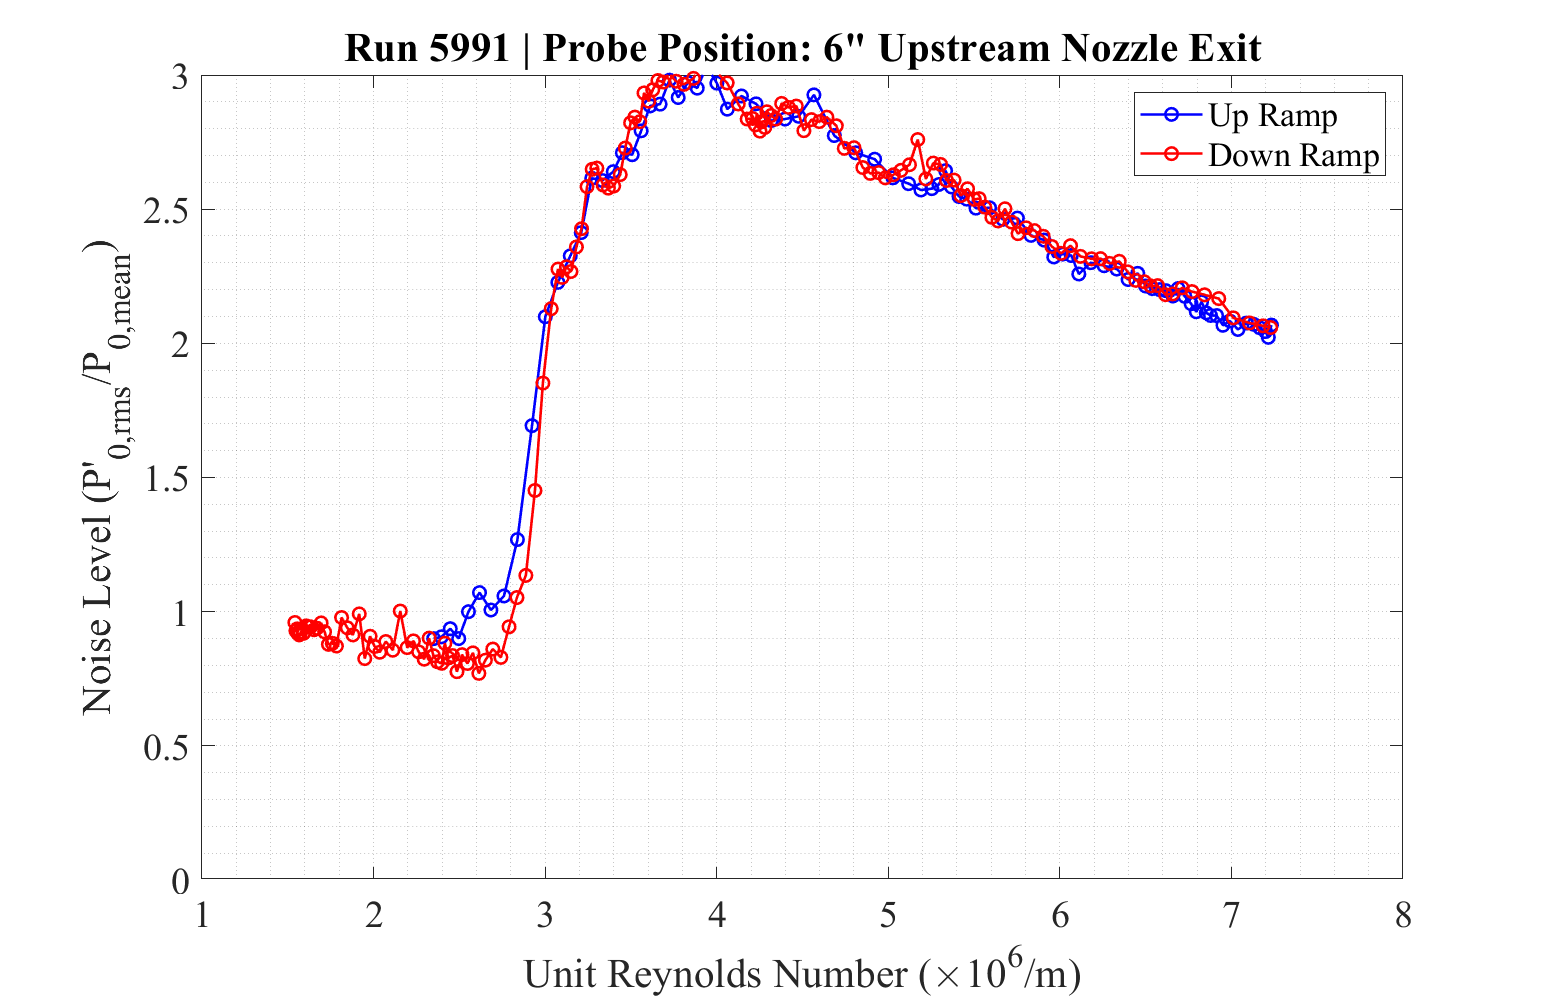
\includegraphics[width=6in]{ace-noise-2024}
    \caption{ACE freestream pressure fluctuations...}
    \label{fig:ace-survey}
\end{figure}

The anticipated characterization test matrix for ACE2.0 is shown in Table \ref{tab:ace2-survey}. The pitot rake will be used to characterize the freestream flow uniformity in the nozzle exit plane and a plane 6 inches upstream. The single pitot probe and hot-wire anemometer will be used to measure the freestream pressure fluctuation and mass flux fluctuation levels, respectively, along the centerline up to 24 inches upstream of the nozzle exit. The runs in each test matrix are divided into a few distinct objectives: (1) uniformity, (2) uncertainty quantification, (3) disturbance levels transition, and (4) hysteresis. The last five runs will be replicates of the first five to better quantify the uncertainty in Mach number, Reynolds number, and flow uniformity. This entire process will be documented so that flow-quality verification tests can be repeated as part of ongoing lab operations.

\begin{figure}[ht!]
    \centering
    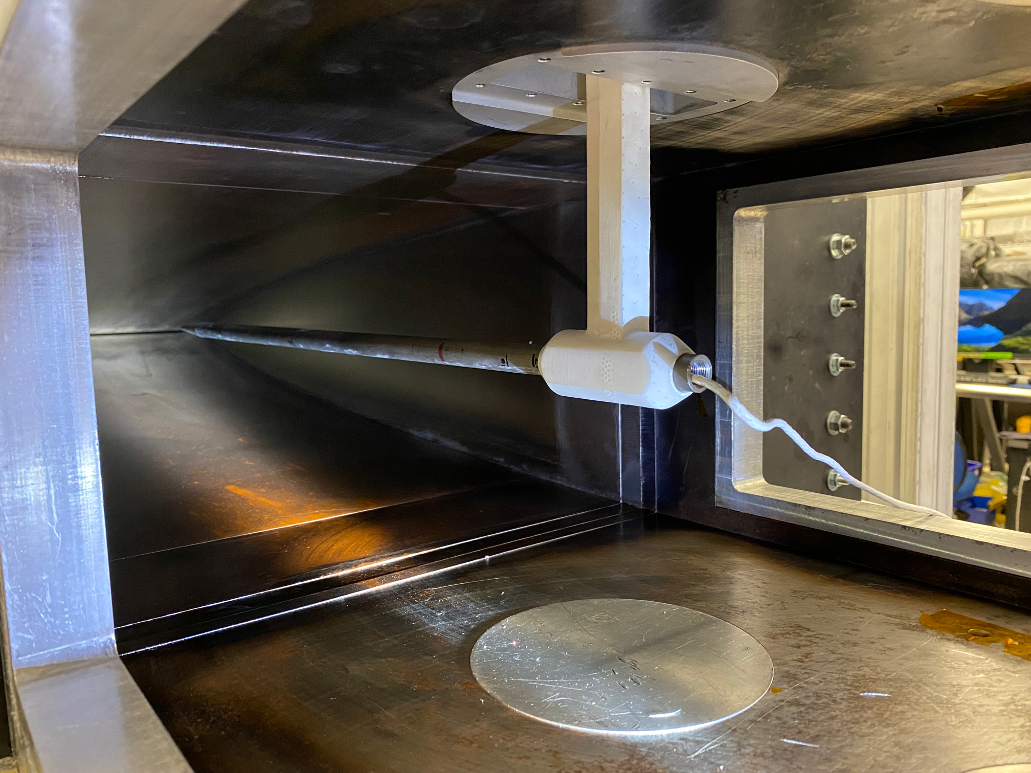
\includegraphics[width=6in]{pitot17}
    \caption{Pitot probe measuring 24 inches upstream of nozzle exit.}
    \label{fig:pitot17}
\end{figure}

% \begin{table}[ht!]
%     \centering
%     \begin{tabular}{|c|c|c|c|c|}
%         \hline
%     \textbf{Run} & \textbf{X (in.)} & \textbf{Y (in.)} & \textbf{Z (in.)} & \textbf{$Re'$ ($\times10^6$)} \\ \hline
%         1 & 0 & 0 & 0 & 2$\to$7$\to$2 \\ \hline
%         2 & -6 & 0 & 0 & 2$\to$7$\to$2 \\ \hline
%         3 & -17 & 0 & 0 & 2$\to$7$\to$2 \\ \hline
%         4 & -24 & 0 & 0 & 2$\to$7$\to$2 \\ \hline
%     \end{tabular}
%     \caption{Test matrix for preliminary noise hysteresis in ACE.}
%     \label{tab:ace-survey}
% \end{table}

% \setcounter{rownum}{0}
% \begin{table}[ht!]
%     \centering
%     \begin{tabular}{|>{\stepcounter{rownum}\therownum}c|c|c|c|c|c|}
%         \hline
%         \multicolumn{1}{|c|}{\textbf{Run}} & \textbf{X (in.)} & \textbf{Y (in.)} & \textbf{Z (in.)} & \textbf{Mach} & \textbf{$Re'$ ($10^6$)} \\ \hline
%         & 0 & 0 & 0 & 6$^*$ & 3$^*$ \\ \hline
%         & 0 & 0 & 0 & 6 & 2$\to$7$\to$2 \\ \hline
%         & 0 & 0 & 0 & 5$\to$8$\to$5 & 3 \\ \hline
%         & 0 & 0 & -3:1:3 & 6 & 3 \\ \hline
%         & 0 & -3 & -3:1:3 & 6 & 3 \\ \hline
%         & 0 & -1.5 & -3:1:3 & 6 & 3 \\ \hline
%         & 0 & 1.5 & -3:1:3 & 6 & 3 \\ \hline
%         & 0 & 3 & -3:1:3 & 6 & 3 \\ \hline
%         & -6 & 0 & 0 & 8 & 2$\to$7$\to$2 \\ \hline
%         & -6 & 0 & 0 & 7 & 2$\to$7$\to$2 \\ \hline
%         & -6 & 0 & 0 & 6 & 2$\to$7$\to$2 \\ \hline
%         & -6 & 0 & 0 & 5 & 2$\to$7$\to$2 \\ \hline
%         & -6 & 0 & 0 & 5$\to$8$\to$5 & 3 \\ \hline
%         & -6 & 0 & -3:1:3 & 6 & 3 \\ \hline
%         & -6 & -3 & -3:1:3 & 6 & 3 \\ \hline
%         & -6 & -1.5 & -3:1:3 & 6 & 3 \\ \hline
%         & -6 & 1.5 & -3:1:3 & 6 & 3 \\ \hline
%         & -6 & 3 & -3:1:3 & 6 & 3 \\ \hline
%         & -17 & 0 & 0 & 6 & 2$\to$7$\to$2 \\ \hline
%         & -17 & 0 & 0 & 5$\to$8$\to$5 & 3 \\ \hline
%         & -24 & 0 & 0 & 6 & 2$\to$7$\to$2 \\ \hline
%         & -24 & 0 & 0 & 5$\to$8$\to$5 & 3 \\ \hline
%         (1) & 0 & 0 & 0 & 6$^*$ & 3$^*$ \\ \hline
%         (4) & 0 & 0 & -3:1:3 & 6 & 3 \\ \hline
%         (5) & 0 & -3 & -3:1:3 & 6 & 3 \\ \hline
%         (6) & 0 & -1.5 & -3:1:3 & 6 & 3 \\ \hline
%         (7) & 0 & 1.5 & -3:1:3 & 6 & 3 \\ \hline
%         (8) & 0 & 3 & -3:1:3 & 6 & 3 \\ \hline
%     \end{tabular}
%     \caption{Test matrix for ACE2.0 characterization with only single pitot.}
%     \label{tab:ace2-survey-norake}
% \end{table}

\setcounter{rownum}{0}
\begin{table}[ht!]
    \centering
    \begin{tabular}{|>{\stepcounter{rownum}\therownum}c|c|c|c|c|c|c|}
        \hline
        \multicolumn{1}{|c|}{\textbf{Run}} & \textbf{X (in.)} & \textbf{Y (in.)} & \textbf{Z (in.)} & \textbf{Mach} & \textbf{$Re'$ ($10^6$)} & \textbf{ Instrument} \\ \hline
        & 0 & -3:1:3 & 0 & 6$^*$ & 3$^*$ & Rake\\ \hline
        & 0 & -3:1:3 & -3:1:3 & 8 & 3 & Rake\\ \hline
        & 0 & -3:1:3 & -3:1:3 & 7 & 3 & Rake\\ \hline
        & 0 & -3:1:3 & -3:1:3 & 6 & 3 & Rake\\ \hline
        & 0 & -3:1:3 & -3:1:3 & 5 & 3 & Rake\\ \hline
        & -6 & -3:1:3 & -3:1:3 & 5 & 3 & Rake\\ \hline
        & -6 & -3:1:3 & -3:1:3 & 6 & 3 & Rake\\ \hline
        & -6 & -3:1:3 & -3:1:3 & 7 & 3 & Rake\\ \hline
        & -6 & -3:1:3 & -3:1:3 & 8 & 3 & Rake\\ \hline
        & 0 & 0 & 0 & 8 & 2$\to$7$\to$2 & Pitot\\ \hline
        & 0 & 0 & 0 & 7 & 2$\to$7$\to$2 & Pitot\\ \hline
        & 0 & 0 & 0 & 6 & 2$\to$7$\to$2 & Pitot\\ \hline
        & 0 & 0 & 0 & 5 & 2$\to$7$\to$2 & Pitot\\ \hline
        & 0 & 0 & 0 & 5$\to$8$\to$5 & 3 & Pitot\\ \hline
        & -6 & 0 & 0 & 5$\to$8$\to$5 & 3 & Pitot\\ \hline
        & -6 & 0 & 0 & 5 & 2$\to$7$\to$2 & Pitot\\ \hline
        & -6 & 0 & 0 & 6 & 2$\to$7$\to$2 & Pitot\\ \hline
        & -6 & 0 & 0 & 7 & 2$\to$7$\to$2 & Pitot\\ \hline
        & -6 & 0 & 0 & 8 & 2$\to$7$\to$2 & Pitot\\ \hline
        & -17 & 0 & 0 & 6 & 2$\to$7$\to$2 & Pitot\\ \hline
        & -17 & 0 & 0 & 5$\to$8$\to$5 & 3 & Pitot\\ \hline
        & -24 & 0 & 0 & 5$\to$8$\to$5 & 3 & Pitot\\ \hline
        & -24 & 0 & 0 & 6 & 2$\to$7$\to$2 & Pitot\\ \hline
        -\stepcounter{rownum}\stepcounter{rownum}\stepcounter{rownum}\stepcounter{rownum}\stepcounter{rownum}\stepcounter{rownum}\stepcounter{rownum}\stepcounter{rownum}\stepcounter{rownum}\stepcounter{rownum}\stepcounter{rownum}\stepcounter{rownum}\stepcounter{rownum}\therownum & \multicolumn{6}{|c|}{\textbf{Repeat runs 10-23 with Hot-wire}} \\ \hline
        -\stepcounter{rownum}\stepcounter{rownum}\stepcounter{rownum}\stepcounter{rownum}\therownum & \multicolumn{6}{|c|}{\textbf{Replicate runs 1-5}} \\ \hline
    \end{tabular}
    \caption{Test matrix for ACE2.0 freestream characterization.}
    \label{tab:ace2-survey}
\end{table}

\subsection{Freestream Uncertainty Quantification}

The process to quantify the uncertainty of the various parameters for this work will closely follow Stephens's et al. \cite{stephens-hubbard} and Curriston's \cite{curriston-dis} approaches by simply focusing on establishing a baseline for the uncertainty and making recommendations for improvement if necessary. The three steps to establish this baseline uncertainty for ACE2.0 will be (1) gather/measure systematic elemental uncertainties, (2) input into a Monte Carlo code along with data reduction equations to simulate systematic uncertainties, and (3) measure repeat data points through a few replicate experiments and calculate random uncertainties.

First, the systematic elemental uncertainties can be gathered and measured from the various sensors, which includes the static pressure transducer, stagnation pressure transducer, stagnation temperature thermocouple, and servo motor internal encoders. Each of these has a predefined manufacturer uncertainty that can be used, but some of these are very conservative and not ideal. The pressure sensors and temperature sensor will be tested against a working standard to measure the true uncertainty, which is often found to be an order of magnitude less than the manufacturer uncertainty \cite{curriston-dis}. The systematic uncertainly of any sensors utilized in future experiments is outside the scope of this work and must be considered when calculating the total uncertainty of measurements in each experiment.

Next, these systematic elemental uncertainties will be propagated through a Monte Carlo simulation along with the specific data reduction equations for the facility. This output will provide the total systematic uncertainty for each parameter of interest, which will be added to the random uncertainty to give the total uncertainty. Additionally, this simulation will also be used provide a sensitivity analysis of the uncertainty to the various input parameters. This will be insightful on how to best improve the uncertainty if necessary.

Finally, repeat data points will be measured by repeatedly settling on and off the set condition for the parameter of interest. While data will be gathered throughout the entire characterization test matrix, runs 1 and 20 will be solely for repeat data measurements. These two runs will provide a direct comparison of replicates that will account for any correlations that were not considered or unquantifiable. The standard deviation of this data will be added in quadrature to the systematic uncertainty to calculate the total uncertainty for each parameter of interest for the freestream flow.

\subsection{Freestream Disturbance Hysteresis}

Dynamic sweeps of both Mach number and Reynolds number will be performed to explore any potential hysteresis effects in either the noise or the control parameters. Specifically, this will be accomplished during the dynamic runs in the characterization test matrix in Table \ref{tab:ace2-survey}. The goal is simply to identify the existence of any hysteresis effects to inform future work within ACE2.0. The Reynolds number sweep runs are necessary to determine the value at which transition occurs, so sweeping the Reynolds number back down will not add any additional work and will be ensure that there is no hysteresis. For the Mach number however, there is no past data to determine the existence of hysteresis, so these runs will establish a baseline. The noise level is known to decrease with an increase in Mach number, so identifying any hysteresis in this will be necessary to inform future experiments.

\section{\textcolor{red}{Mach Trajectory and Potential Hysteresis} Proof of Concept Experiment}

This objective will primarily serve as a demonstration of the capabilities for ACE2.0 and will also provide preliminary insight into the hysteretic behavior of dynamic Mach number experiments. The flow characteristic that will be specifically explored in this research will be shock interactions using schlieren. The goal will be to observe hysteresis in the transition from regular reflection to Mach reflection by varying the Mach number. The challenge of this is that the only facilities that have successfully produced this hysteresis had low freestream disturbance levels and an open-jet test section, while ACE2.0 has a closed test section and is not considered a "quiet" facility. In order to provide the best conditions for hysteresis to be observed, these experiments will be performed at higher Mach numbers and a lower unit Reynolds number where freestream disturbance levels are lowest.

The experiments will be based on the methodologies and results from Durand et al. \cite{durand} and Tao et al. \cite{tao} in addition to the experimental setup of Mai \cite{mai-dis}. The Mach number will be varied across either the Von Neumann condition or the detachments criteria to force the transition from regular reflection to Mach reflection or vice versa. In order to choose the wedge angle and Mach number range for each experiment, Figure \ref{fig:dual} was created following the processes shown by Mouton \cite{mouton} for each condition. The basic parameters across an oblique shock shown in Figure \ref{fig:detachment} are given as a function of the Mach number in region x $\left(M_x\right)$, the shock angle ($\alpha$), and the ratio of specific heats ($\gamma$). 

\textcolor{red}{Too much in the weeds. Reword as just process without all the equations}

The pressure ratio is 

\begin{equation}
    \xi \left(M_x,\alpha\right) = \frac{P}{P_x} = \frac{2 \gamma M_x^2 \sin^2{\alpha} - (\gamma-1)}{\gamma+1}
\end{equation}

\noindent The flow deflection angle (wedge angle) and Mach number are given as
\begin{equation}
    \theta \left(M_x,\alpha\right) = \cot^{-1}{\left[ \left(\frac{(\gamma+1) M_x^2}{2\left(M_x^2 \sin^2{\alpha} - 1\right)}\right) \tan{\alpha} \right]}
\end{equation}
\begin{equation}
    M \left(M_x,\alpha\right) = \sqrt{\frac{(\gamma+1)^2 M_x^4 \sin^2{\alpha} - 4\left(M_x^2 \sin^2{\alpha} - 1\right)\left(\gamma M_x^2 \sin^2{\alpha} + 1\right)}{\left[2 \gamma M_x^2 \sin^2{\alpha} - (\gamma-1)\right]\left[(\gamma-1) M_x^2 \sin^2{\alpha} + 2\right]}}
\end{equation}

The shock angle when the flow deflection angle is maximum is given by setting $\frac{\partial \theta}{\partial \alpha} = 0$, resulting in
\begin{equation}
    \alpha^{\theta_{max}}(M_x) = \sin^{-1}{\sqrt{(\gamma+1)\frac{M_x^2 - \frac{4}{\gamma+1} + \sqrt{M_x^4 + 8\frac{\gamma-1}{\gamma+1}M_x^2 + \frac{16}{\gamma+1}}}{4 \gamma M_x^2}}}
\end{equation}

For the detachment condition shown in Figure \ref{fig:detachment}
\begin{equation}
    M_{1,D} = M(M_{\infty},\alpha_D)
\end{equation}
\begin{equation}
    \theta(M_{\infty},\alpha_D) = \theta\left(M_{1,D},\alpha^{\theta_{max}}(M_{1,D})\right)
\end{equation}

Solving this for $\alpha_D$ results in a fifth-order polynomial in $\sin^2{\alpha_D}$
\begin{equation}
    D_0 + D_1 \sin^2{\alpha_D} + D_2 \sin^4{\alpha_D} + D_3 \sin^6{\alpha_D} + D_4 \sin^8{\alpha_D} + D_5 \sin^{10}{\alpha_D} = 0
\end{equation}

where
\begin{align*}
    D_0 =& -16 \\
    D_1 =& \; 32M_{\infty}^2 - 4M_{\infty}^4 - 48M_{\infty}^2\gamma - 16M_{\infty}^4\gamma + 16\gamma^2 - 16M_{\infty}^4\gamma^2 \\
         & + 16M_{\infty}^2\gamma^3 + 4M_{\infty}^4\gamma^4 \\
    D_2 =& - 16M_{\infty}^4 + 4M_{\infty}^6 - M_{\infty}^8 + 104M_{\infty}^4\gamma + 16M_{\infty}^6\gamma - 4M_{\infty}^8\gamma \\
         & - 64M_{\infty}^2\gamma^2 - 32M_{\infty}^4\gamma^2 + 8M_{\infty}^6\gamma^2 - 6M_{\infty}^8\gamma^2 -56M_{\infty}^4\gamma^3 \\
         & - 16M_{\infty}^6\gamma^3 - 4M_{\infty}^8\gamma^3 - 12M_{\infty}^6\gamma^4 - M_{\infty}^8\gamma^4 \\
    D_3 =& \; M_{\infty}^8 - 64M_{\infty}^6\gamma + 4M_{\infty}^8\gamma + 96M_{\infty}^4\gamma^2 +64M_{\infty}^6\gamma^2 + 14M_{\infty}^8\gamma^2 \\
         & + 64M_{\infty}^6\gamma^3 +20M_{\infty}^8\gamma^3 + 9M_{\infty}^8\gamma^4 \\
    D_4 =& \; 8M_{\infty}^8\gamma - 64M_{\infty}^6\gamma^2 - 32M_{\infty}^8\gamma^2 - 24M_{\infty}^8\gamma^3 \\
    D_5 =& \; 16M_{\infty}^8\gamma^2 \\
\end{align*}

This equation is solved numerically for Mach numbers greater than unity, and only one solution for each $\sin^{2}{\alpha_D}$ exists that is real and bounded between zero and one. The values of $\theta_D(M) = \theta\left(M_{\infty},\alpha_D\right)$ solved for freestream Mach numbers from 2 to 9 yields the upper curve in Figure \ref{fig:dual}.

For the Von Neumann condition shown in Figure \ref{fig:von-neumann}
\begin{equation}
    M_{1,V} = M(M_{\infty},\alpha_V)
\end{equation}
\begin{equation}
    \xi\left(M_{\infty},\frac{\pi}{2}\right) = \xi\left(M_{\infty},\alpha_V\right) \xi\left(M_{1,V},\alpha_{1,V}\right)
\end{equation}
\begin{equation}
    \frac{2 \gamma M_{1,V}^2 \sin^2{\alpha_{1,V}} - (\gamma-1)}{\gamma+1} = \frac{\xi\left(M_{\infty},\frac{\pi}{2}\right)}{\xi\left(M_{\infty},\alpha_V\right)}
\end{equation}
\begin{equation}
    \alpha_{1,V} = \sin^{-1}{\sqrt{\frac{(\gamma-1)+(\gamma+1)\frac{\xi\left(M_{\infty},\frac{\pi}{2}\right)}{\xi\left(M_{\infty},\alpha_V\right)}}{2 \gamma M_{1,V}^2}}}
\end{equation}

The solution for $\alpha_{1,V}$ is found numerically by solving the equation
\begin{equation}
    \theta\left(M_{\infty},\alpha_V\right) = \theta\left(M_{1,V},\alpha_{1,V}\right) 
\end{equation}

The values of $\theta_V(M) = \theta\left(M_{\infty},\alpha_V\right)$ solved for freestream Mach numbers from 2.2 to 9 yields the lower curve in Figure \ref{fig:dual}.

\begin{figure}[ht!]
    \centering
    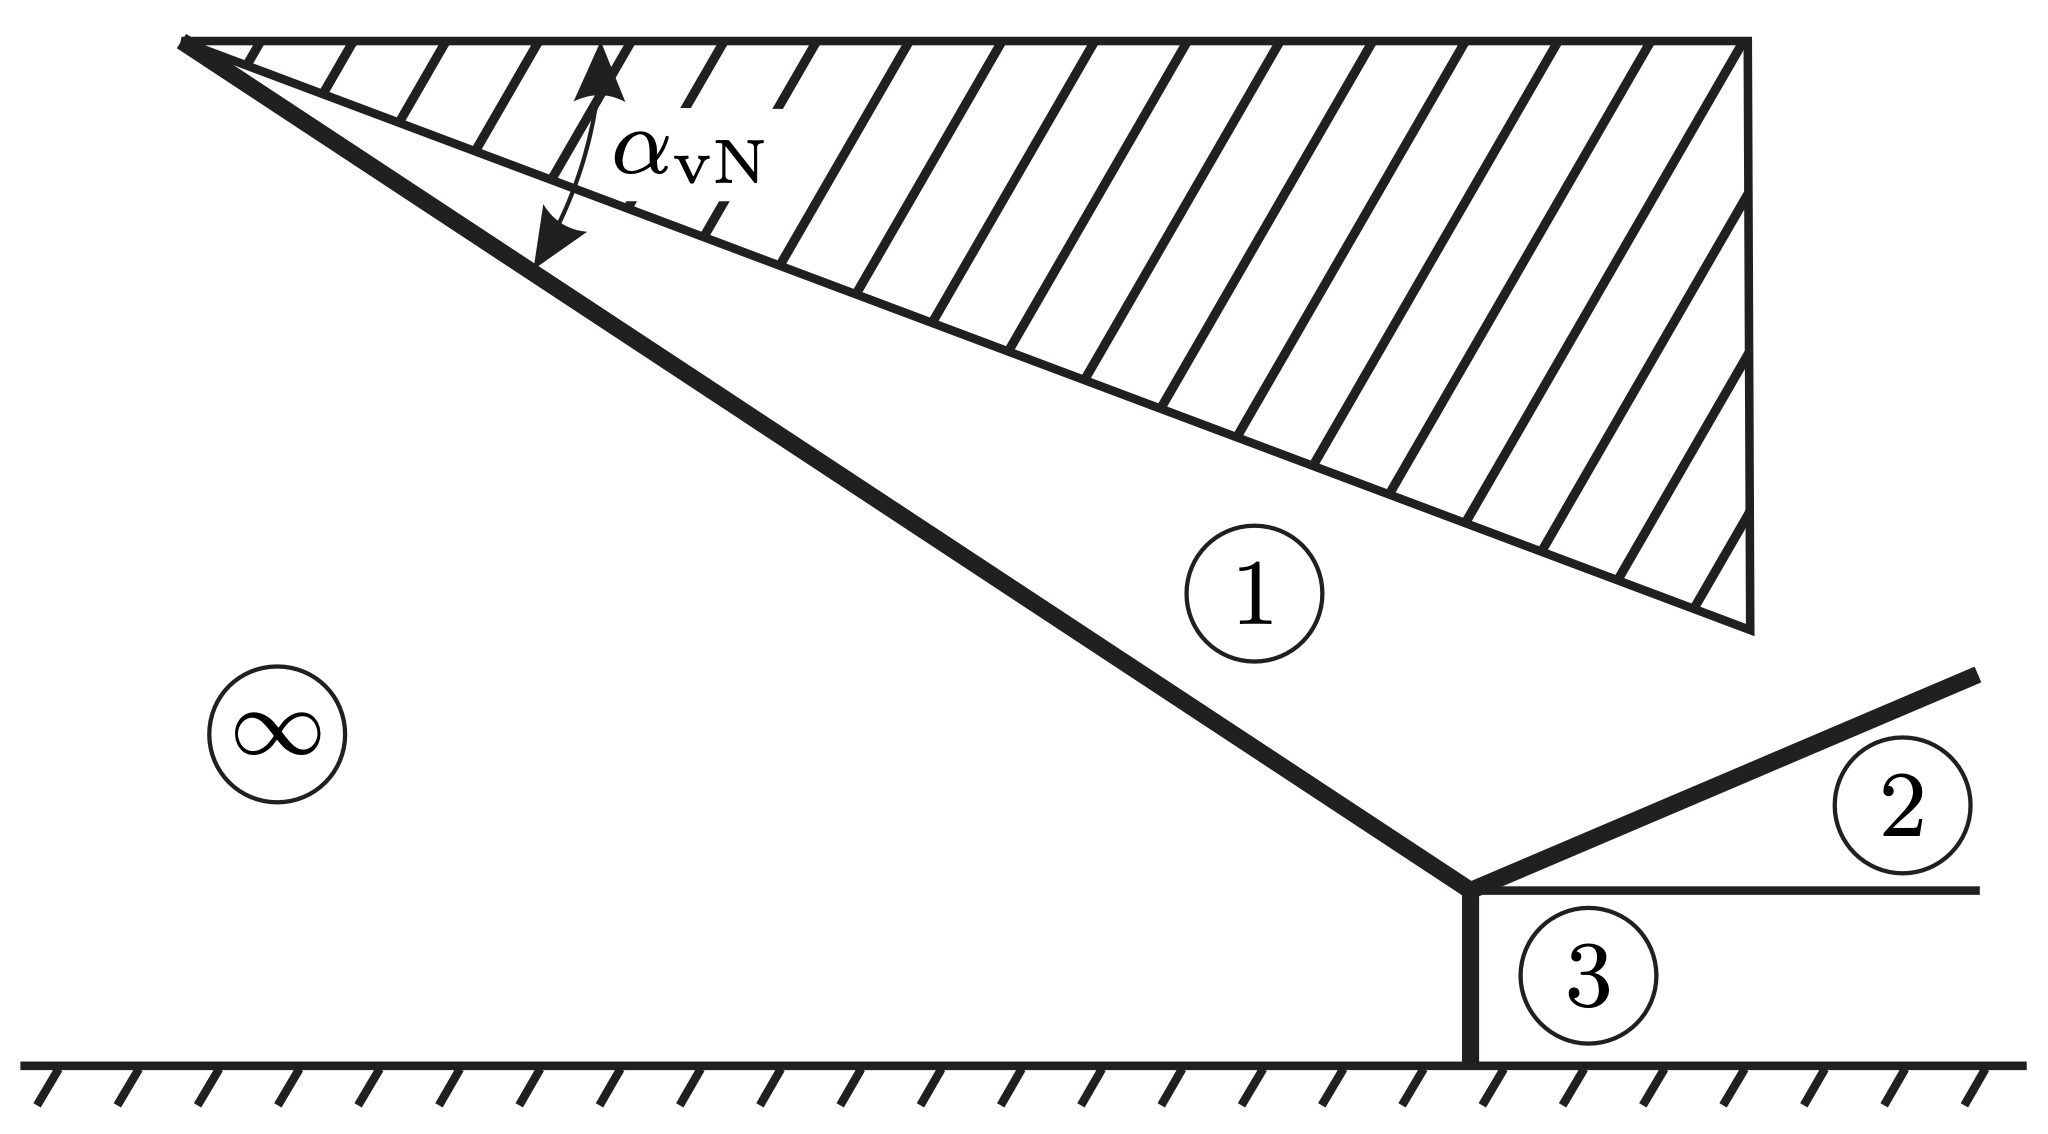
\includegraphics[width=5in]{detachment}
    \caption[Flow over wedge resulting in regular reflection of shock]{Flow over wedge resulting in regular reflection of shock \cite{mouton}}
    \label{fig:detachment}
\end{figure}

\begin{figure}[ht!]
    \centering
    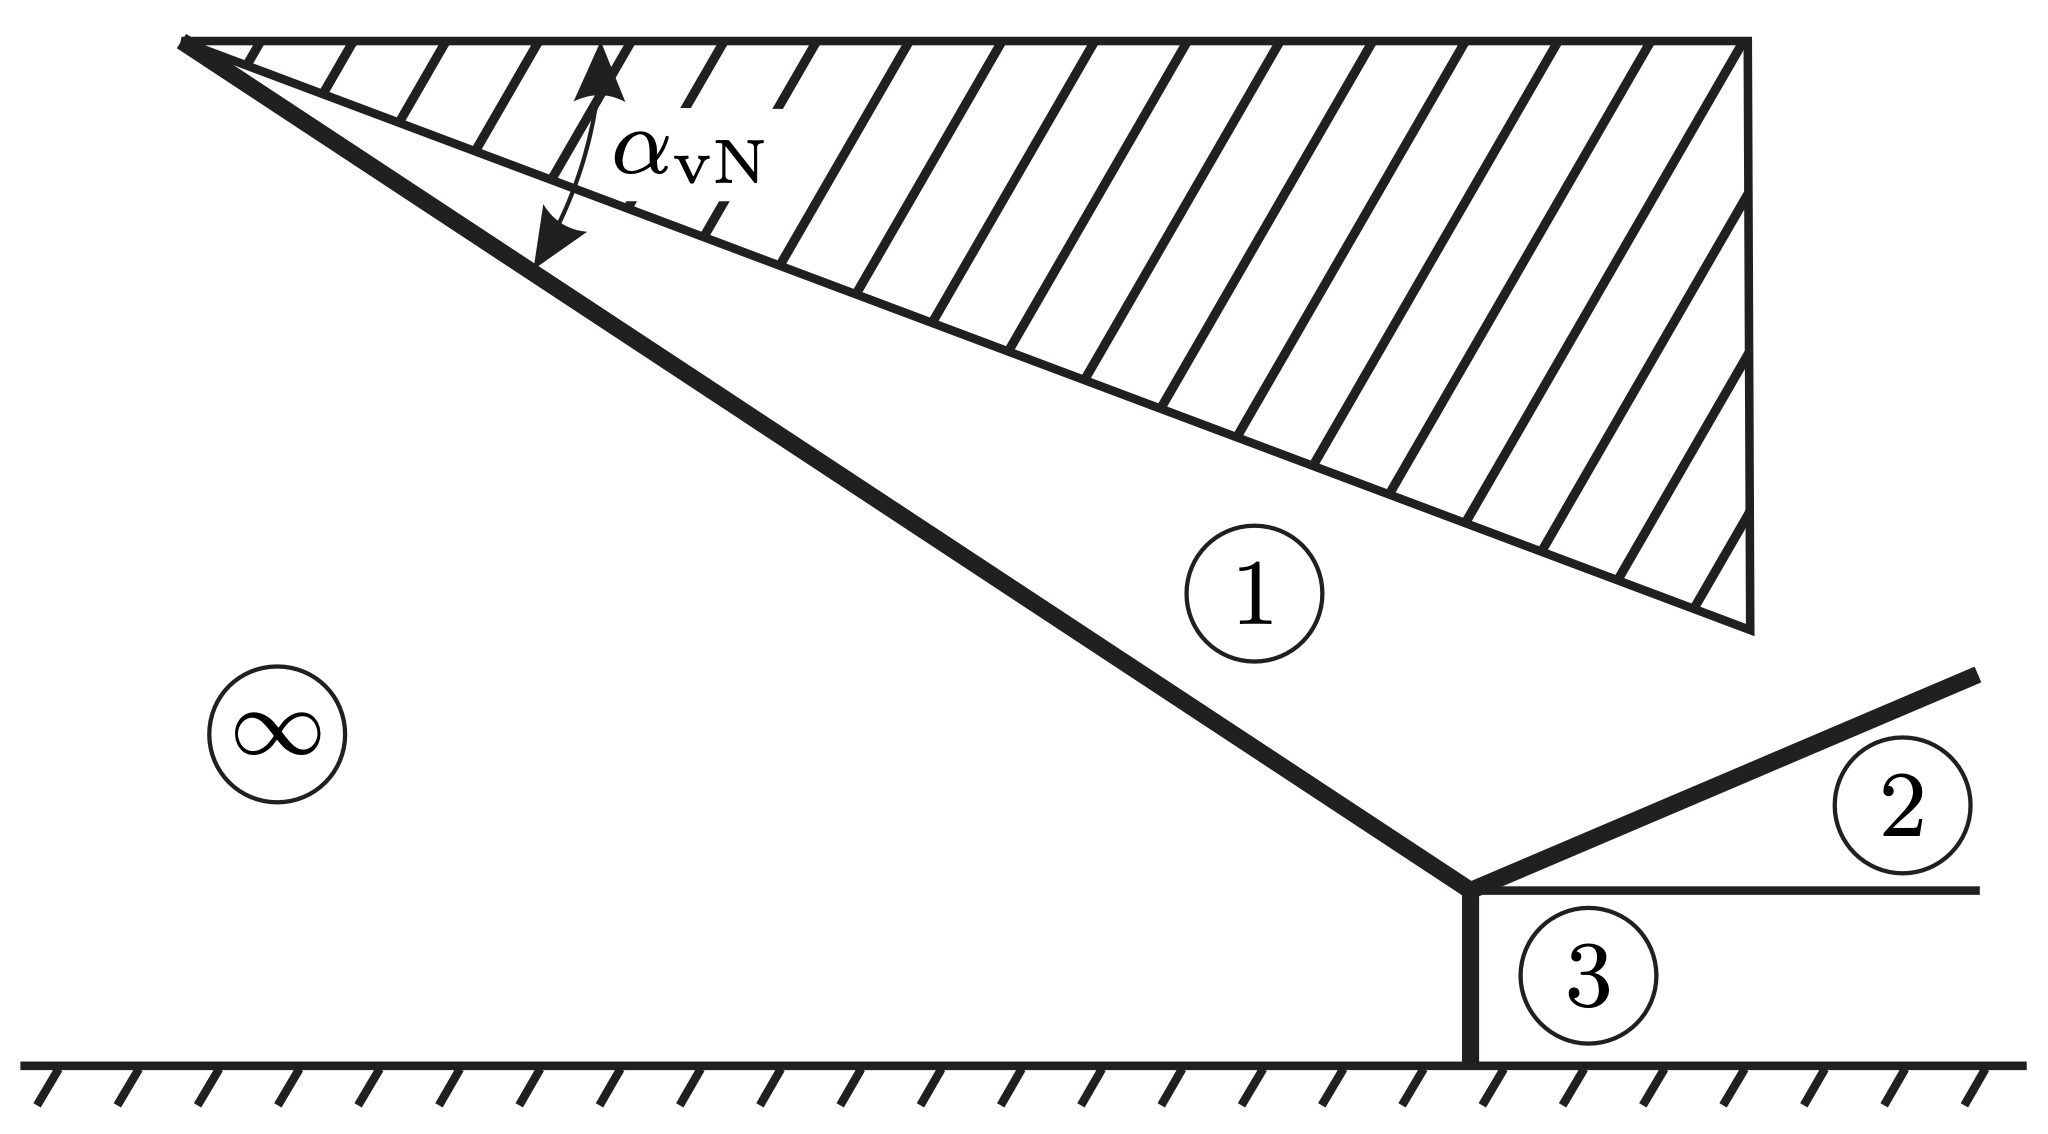
\includegraphics[width=5in]{von-neumann}
    \caption[Flow over wedge resulting in Mach reflection of shock]{Flow over wedge resulting in Mach reflection of shock \cite{mouton}}
    \label{fig:von-neumann}
\end{figure}

The two experimental setups are shown as A and B. For A, the wedge angle is 30$\degree$ and the Mach number range is 7 to 8. For B, the wedge angle is 20.3$\degree$ and the Mach number range is 6 to 8. For both paths, the Mach number will start at the point in the dual solution domain, decrease across either the detachment condition or the Von Neumann condition, and then increase back into the dual solution domain (i.e. AA'A, BB'B). The reverse of these will also be explored if hysteresis is not observed initially.

The physical model for these experiments will be very similar to the double wedge setup used by Mai \cite{mai-dis} in ACE as shown in Figure \ref{fig:wedges}. If 3D printing with Rigid 10K produces an acceptable leading edge, then a pair will be printed for each angle needed. If future research will utilize this double wedge setup, then a hinged mechanism will be designed and fabricated to use a single pair of wedges for any desired angle.

\begin{figure}[ht!]
    \centering
    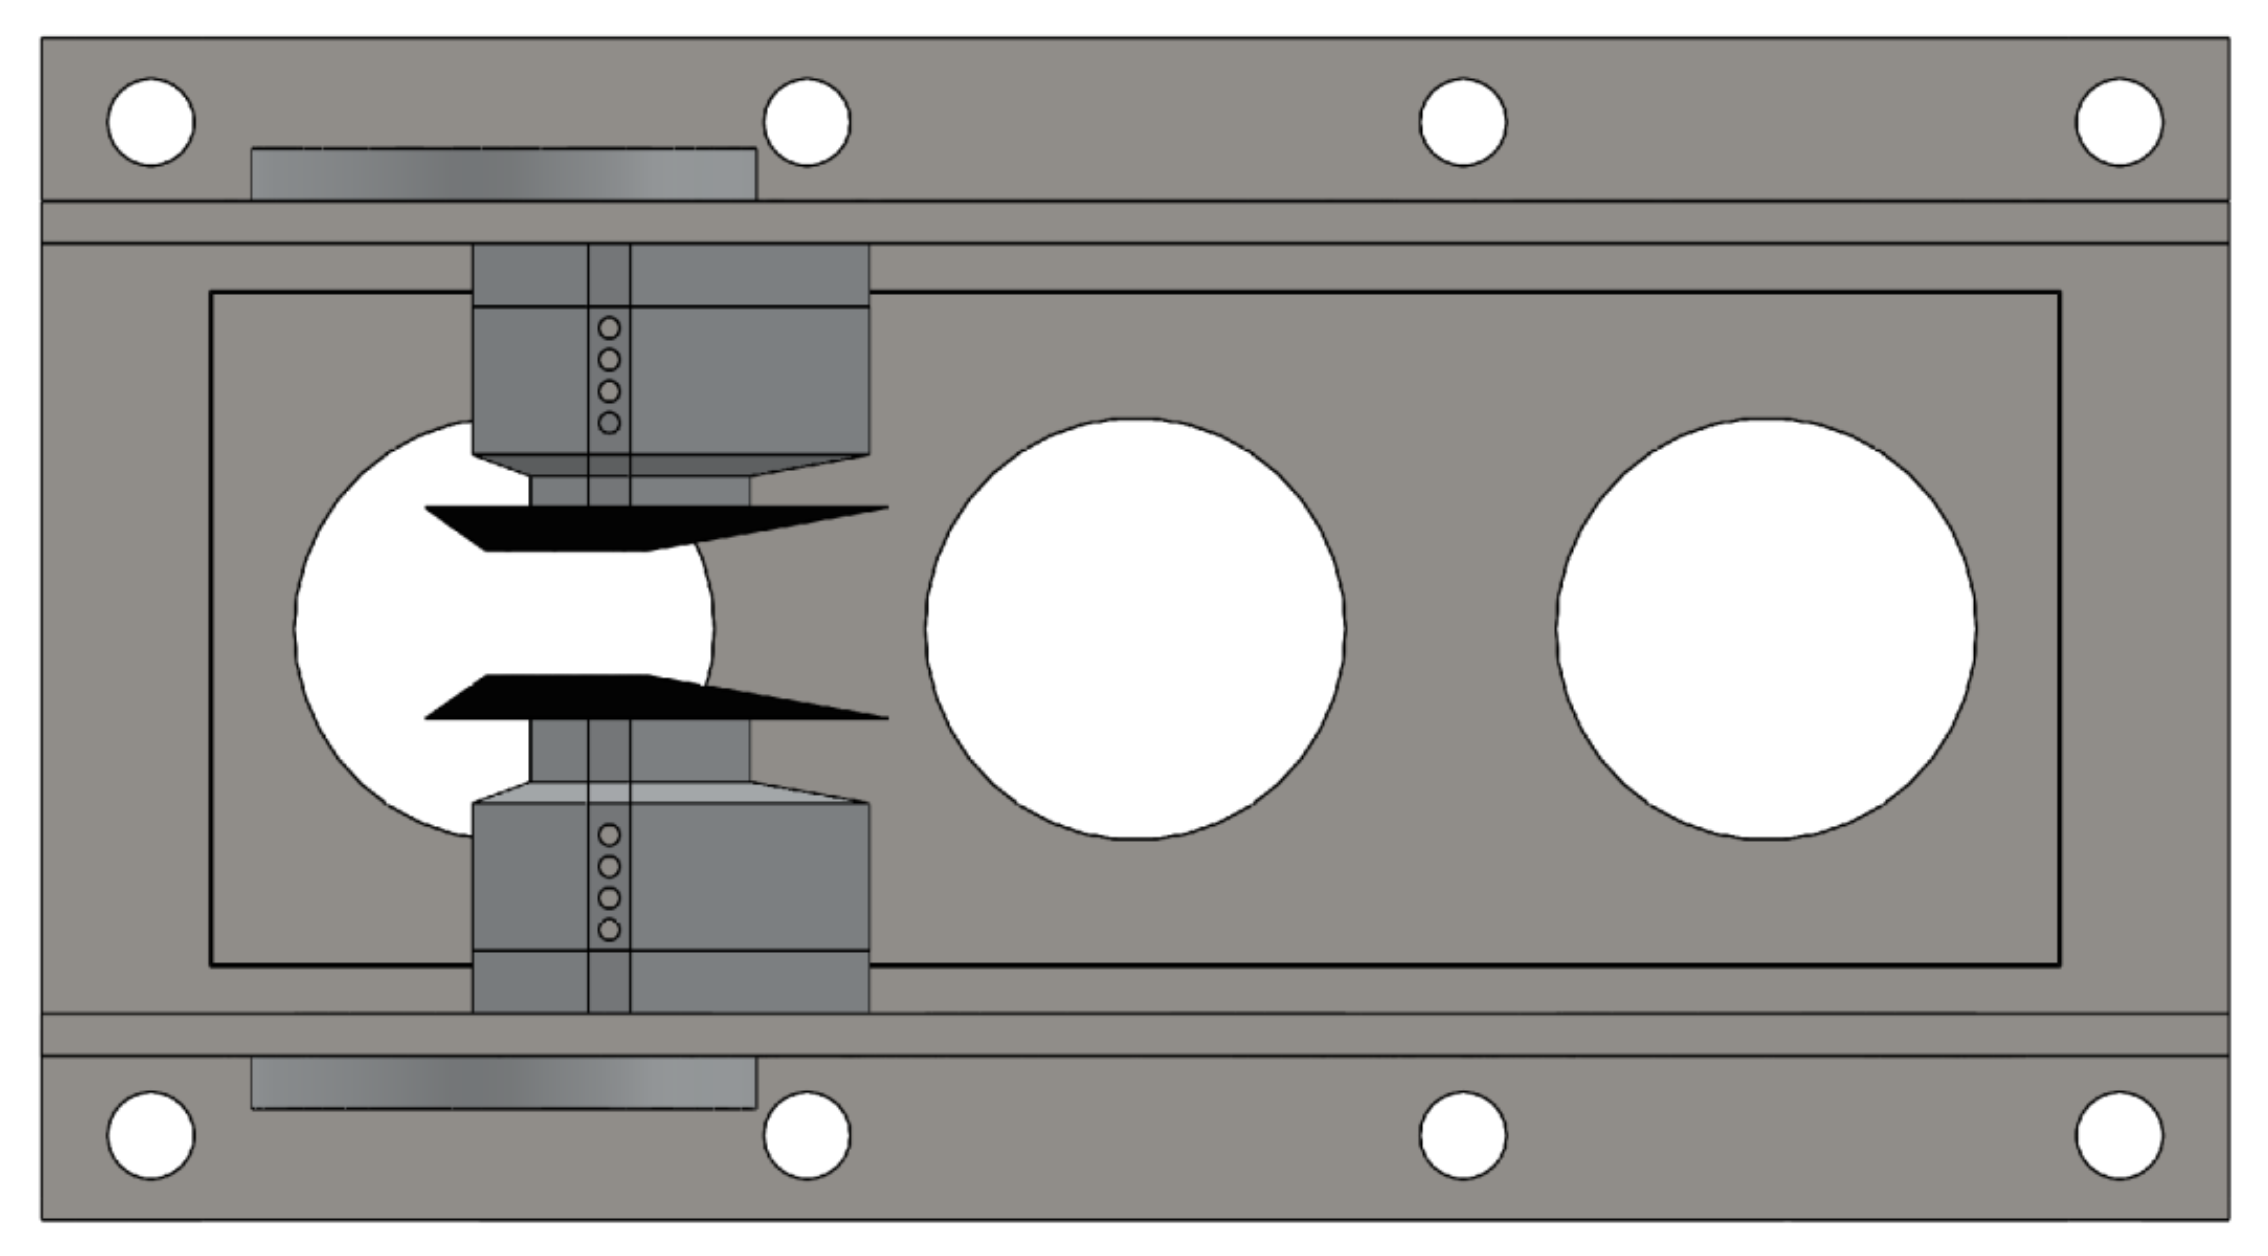
\includegraphics[width=6in]{wedges}
    \caption[Double wedge setup]{Double wedge setup \cite{mai-dis}}
    \label{fig:wedges}
\end{figure}


\begin{figure}[ht!]
    \centering
    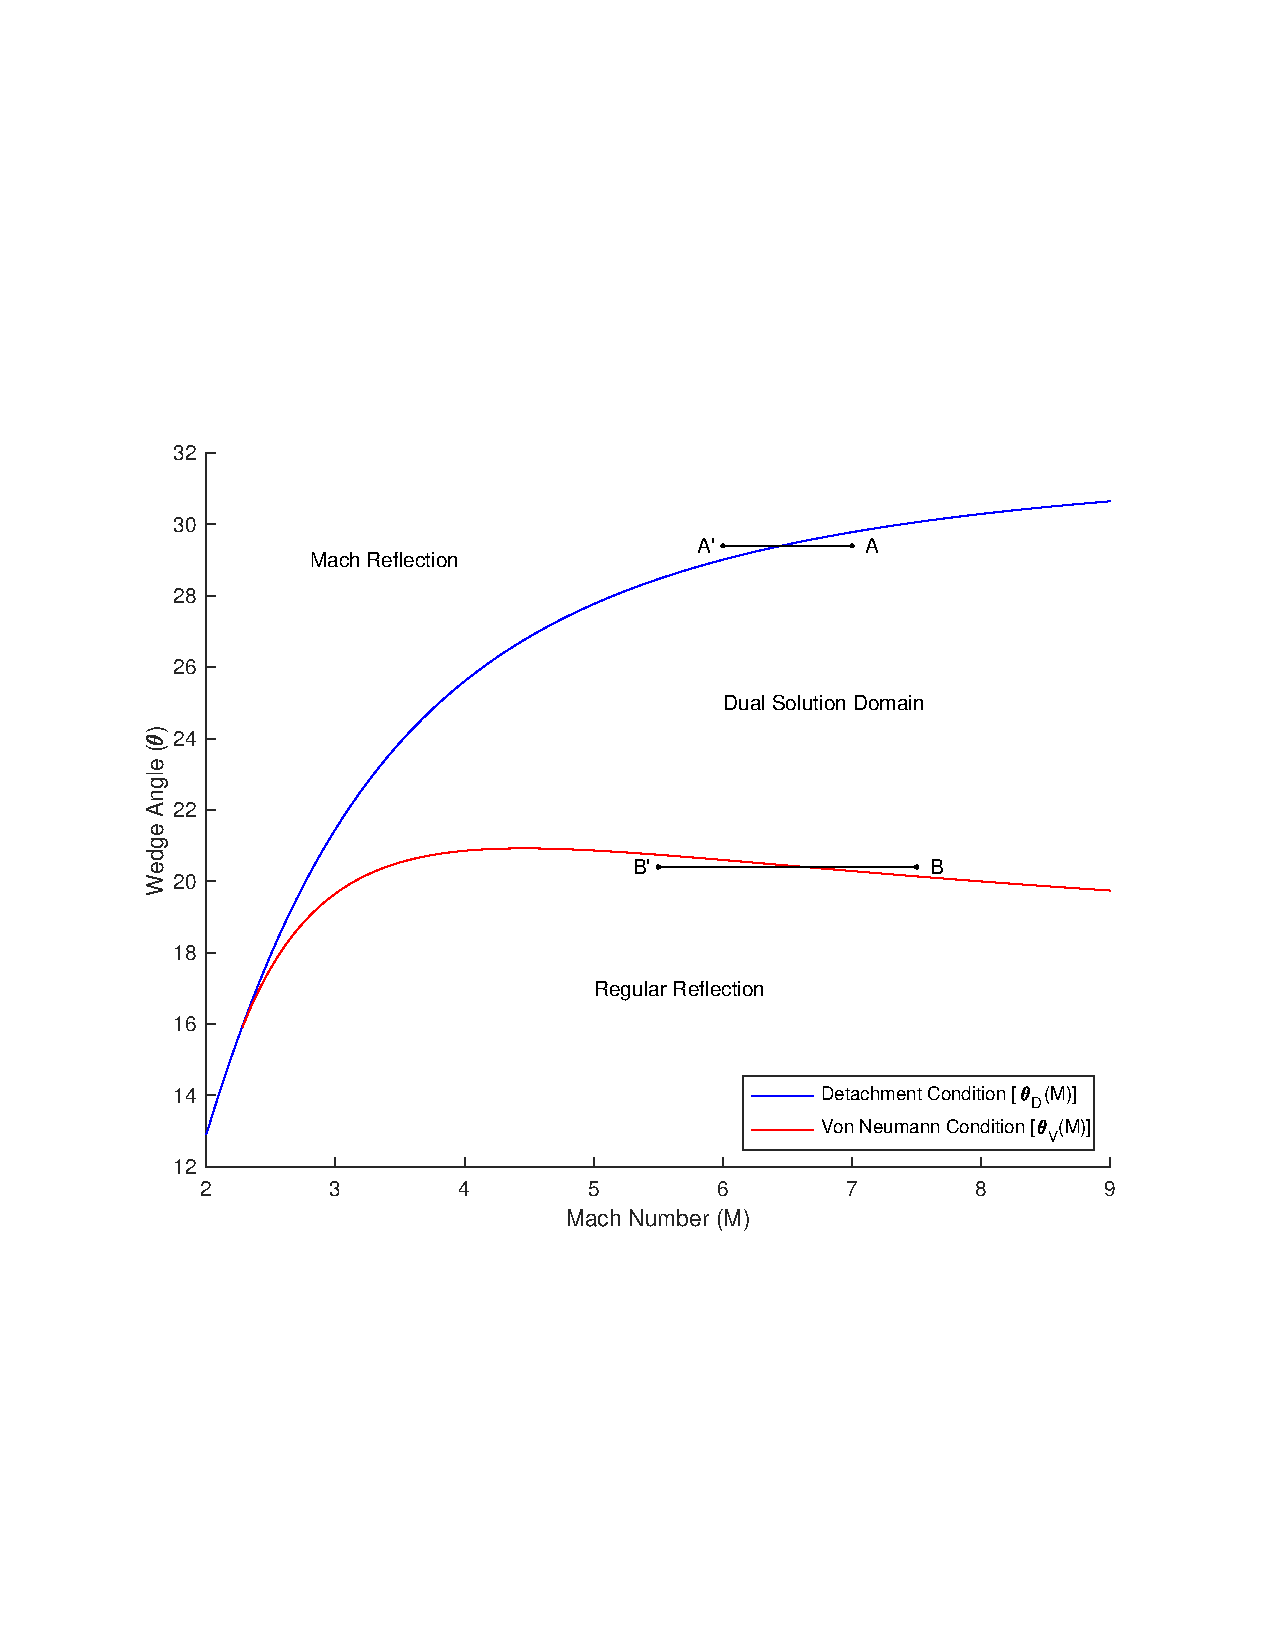
\includegraphics[trim={70 200 70 200},clip,width=6in]{dual.pdf}
    \caption{Shock wave reflection configuration domains for Mach number and wedge angle.}
    \label{fig:dual}
\end{figure}

The expected results should appear similar to the numerical results from Ben-Dor et al. \cite{ben-dor-1}, Durand et al. \cite{durand}, and Tao et al. \cite{tao} with an example shown in Figure \ref{fig:shock-hysteresis}. Although the Mach number range and wedge angle are different, the hysteresis should be the same for the chosen paths in this experiment. The path in Figure \ref{fig:shock-hysteresis} is representative of path AA'A, which crosses the detachment condition. There have not been any simulations published that cross the Von Neumann condition by varying the Mach number, so path B will be explored secondary to path A.

In either case, the final objective will be to guide future experiments by determining if ACE2.0 is capable of reproducing the hysteresis in shock interactions or incapable due to freestream noise. 

\begin{figure}[ht!]
    \centering
    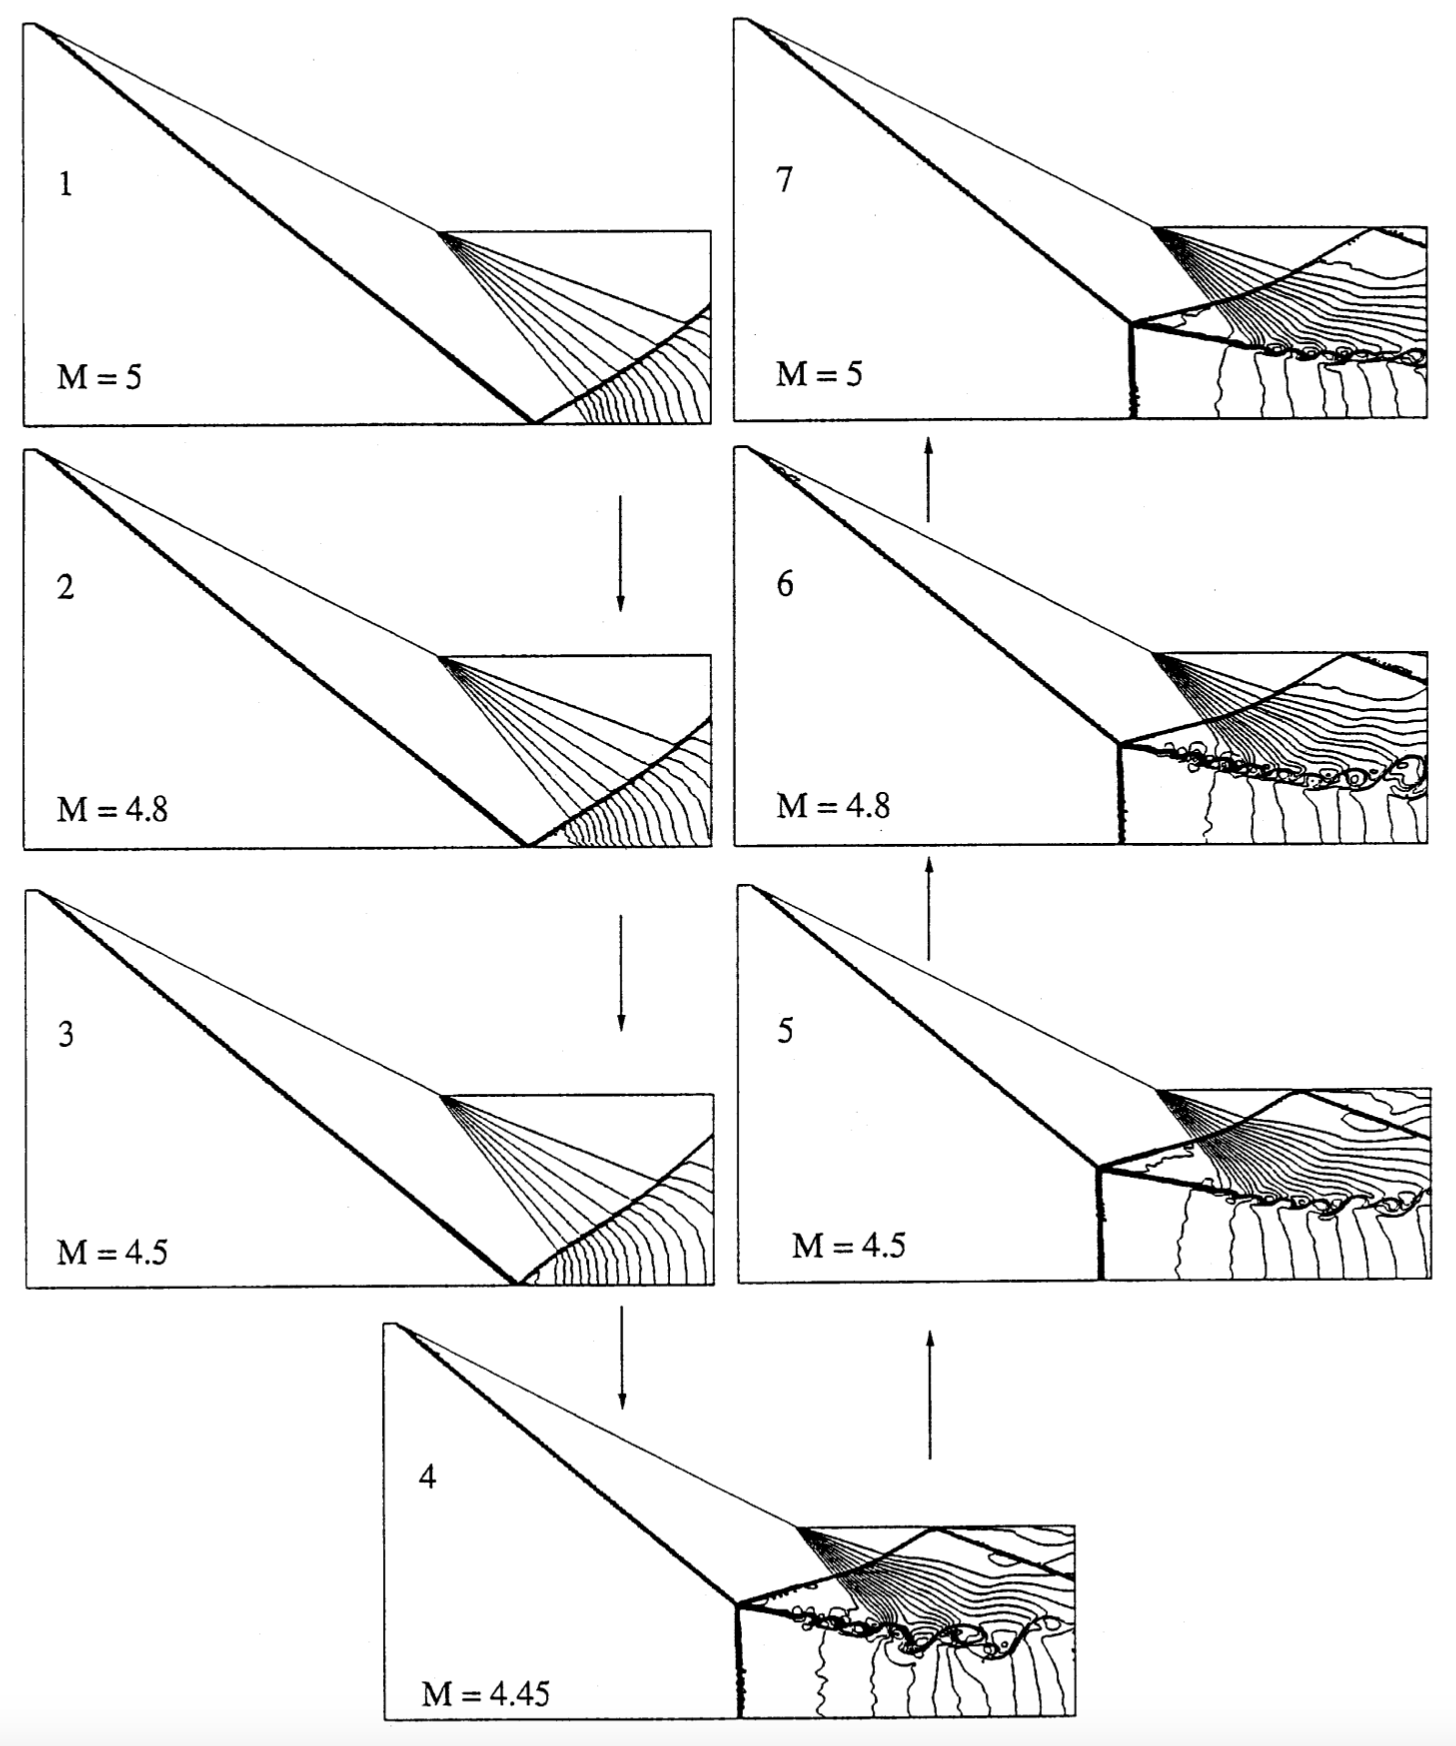
\includegraphics[width=6in]{shock-hysteresis}
    \caption[Mach-number-varitation-induced hysteresis for 27$\degree$ wedge]{Mach-number-variation-induced hysteresis for 27$\degree$ wedge \cite{ben-dor-1}}
    \label{fig:shock-hysteresis}
\end{figure}



